%======================================================
% Technische Universitaet Darmstadt
% Fachbereich Elektrotechnik und Informationstechnik
% Fachbereich Informatik (Zweitmitglied)
% Fachgebiet Multimedia Kommunikation (KOM)
% Prof. Dr.-Ing. Ralf Steinmetz
%======================================================
% Template for Theses
% VERSION 1.0 (October 2009)
% Use pdfLaTeX (other possible, but not supported)
% Contact at KOM: Andr\'e Miede (andre.miede@kom...)
%======================================================
% Official TUD-LaTeX-files have to be installed:
% http://exp1.fkp.physik.tu-darmstadt.de/tuddesign/
% Refer to the manuals and forum for details
%======================================================
\documentclass[longdoc,colorbacktitle=tud1c,accentcolor=tud1c,11pt,paper=a4,exercise]{tudexercise}
%======================================================
% colorback = Bereich unter Titel mit Hintergrundfarbe
% colorbacktitle = Titel mit Hintergrundfarbe (Akzent)
% KOM-Blau = accentcolor=tud1b		
% Grau = accentcolor=tud0a
% blackrule fuer schwarze Leiste
% nochapterpage = do not start chapters on new page 
% oneside = print only on one side of the page
%======================================================

%======================================================
% General package loading and definitions
%======================================================
\usepackage[utf8]{inputenc}
\usepackage{textcomp} 
\usepackage{hyperref}
\usepackage{graphicx}
\usepackage{enumerate}
\usepackage{ulem}


\setlength{\parskip}{0.3cm}
\setlength{\parindent}{0cm}


%\usepackage[english]{babel}
\usepackage{xspace}
\usepackage[fleqn]{amsmath} % math environments and more by the AMS 
\usepackage{listings}
\newcounter{dummy} % necessary for correct hyperlinks (to index, bib, etc.)
\newcommand{\myfloatalign}{\centering} % how all the floats will be aligned


%\Show TODO
\newcommand{\todo}[1]{{\large \textcolor{red}{ToDo:} \large \textcolor{red}{#1}}}

%\DONT Show TODO
%\newcommand{\todo}[1]{}

\newcommand {\corr}[2]{\textcolor{red}{\sout{#1}}  \textcolor{green}{#2} }

 %\newenvironment{hint}{  \setkomafont{minisec}{ \textbf{Hint:}\normalfont\bfseries}   \begin{addmargin}{0.5em}  \minisec{\hspace*{-0.5em}\vspace*{0em}}   }{   \end{addmargin}   \vspace{.0ex} }

\title{Modeling Wizards Master Class 2012}
\subtitle{eMoflon Project Presentation}
\institution{ES TU Darmstadt}
%========\chapter{Background}==============================================
% MAIN DOCUMENT STARTS HERE
%======================================================
\begin{document}
%======================================================
\maketitle
	


\section{Background}
 
Our goal is to give a hands-on introduction to metamodeling and graph transformations using our tool eMoflon. 
Therefore, we have chosen the concrete example of implementing a textual DSL. 

More specifically you will learn how to
\begin{itemize}
  \item specify the semantics of the textual DSL, define operations for statically validating the DSL using programmed graph transformation, and
  \item use this specification to generate an interpreter for the DSL.
\end{itemize} 

 
\subsection{The DSL}
The example DSL is a specification language for automated software build processes (similar to make or ant).

An instance written in the DSL that exemplifies the build process of our tool eMoflon can be found in Figure~\ref{fig: Example instance written in the DSL}. 
Such an instance is composed of a system module, a container for other modules that in turn contains an arbitrary number of tasks. 
Note that the folder structure is also part of the DSL. A task consists of a \texttt{run()} statement that represents some internal operations that are performed whenever the task is invoked. 
Additionally, a task can invoke other tasks within the \texttt{run()} statement. For example, the task \texttt{deploy\_to\_server} invokes the tasks \texttt{visual\_studio\_project} and \texttt{build\_update\_site}. 
As the task \texttt{visual\_studio\_project} reside in a different module, it is ensured that the corresponding location (the module) is known to the task by the import statement. 
When a task is run the partial order of task invocations is derived on the fly.
\begin{figure}[h]
\begin{center} 
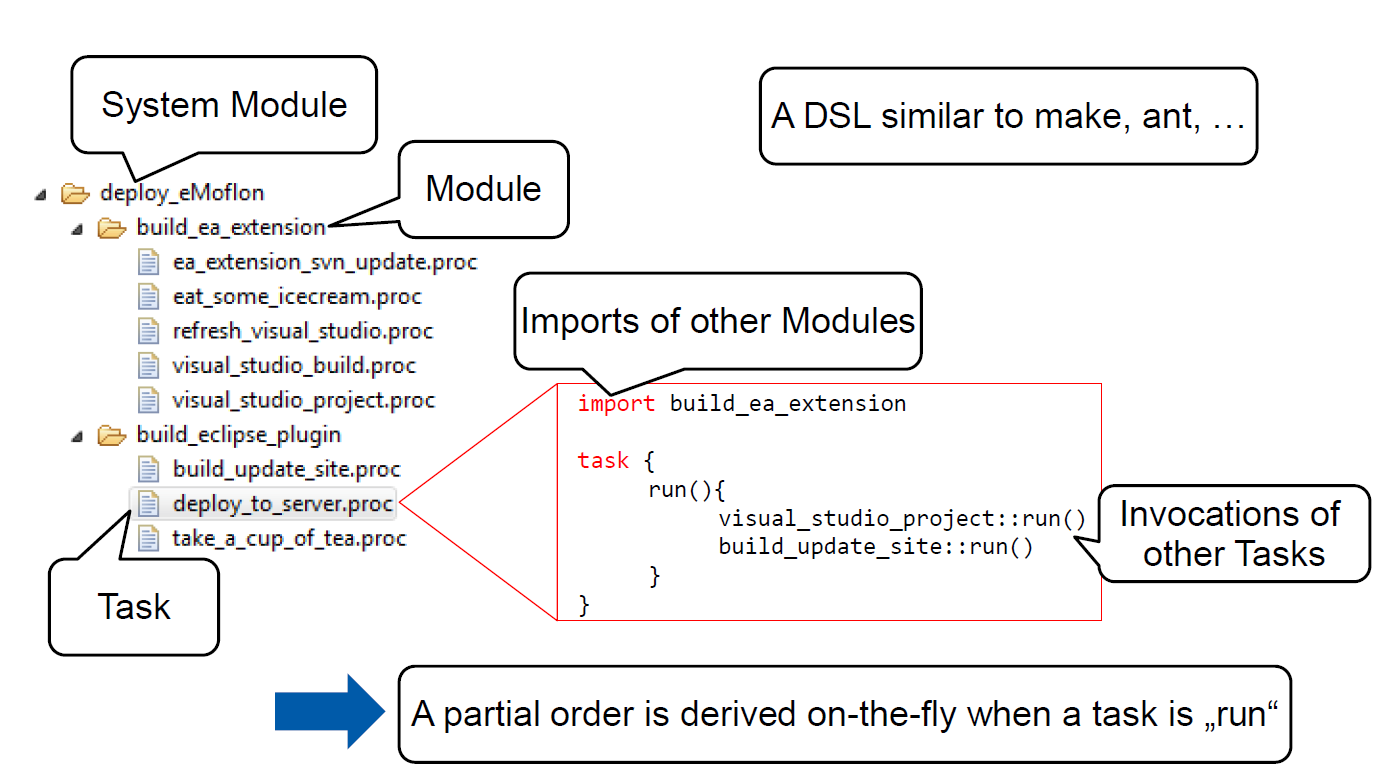
\includegraphics[width=0.5\textwidth]{figures/DSL.png} 
\end{center}
\caption{Example instance written in the DSL}
\label{fig: Example instance written in the DSL}
\end{figure}  

\subsection{The workflow for compiling and validating instances}
\label{sec: The workflow for compiling and validating instances}
The workflow for compiling and validating instances written in the DSL is depicted in Figure~\ref{fig: Workflow to Compile the DSL}.  


\begin{figure}[ht]
\begin{center} 
\includegraphics[width=0.5\textwidth]{figures/workflow.png} 
\end{center}
\caption{Workflow for compiling the DSL}
\label{fig: Workflow to Compile the DSL}
\end{figure}  




It consists of the following steps:
\begin{enumerate}[1)]
 \item \textbf{Text-to-Tree:}  The textual representation of an instance written in the DSL is parsed using a parser generated with ANTLR. The result is a tree representation of the instance. 
 \item \label{enumF2}\textbf{Tree-to-Model:} This tree is transformed to an instance of the Process Language metamodel using a transformation specified by a Triple Graph Grammar (TGG).
 \item \textbf{Model-to-Model:} Based on this representation (abstract syntax), the validation and (if necessary) correction operations are specified by Story Driven Modeling (SDM). Furthermore, the interpreter that runs the tasks in the defined order is specified here.
 \item \textbf{Model-to-Tree:} The corrected instances are transformed back to the tree representation using a transformation specified by the same TGG as used for the Tree-to-Model transformation.
 \item \textbf{Tree-to-Model:} Finally, the tree is unparsed using an unparser generated with ANTLR. 
\end{enumerate}




\subsection{Installation} 
Before you start, make sure that our tool eMoflon and ANTLR (a lexer parser generator) are installed.
Our tutorial\footnote{You can download the tutorial at \url{www.moflon.org}} contains detailed instructions on how to install eMoflon and set up ANTLR (see Chapter~2 and Chapter~5.1, respectively).



\subsection{Project Structure}
In order to facilitate the introduction into modeling with eMoflon, a workspace containing the basic building blocks can be downloaded\footnote{Eclipse Workspace: \url{http://www.moflon.org/fileadmin/download/eMoflon/ProcessLanguageWorkspace.zip}}. For example, it contains the parser and unparser and the sample instance presented in Figure \ref{fig: Example instance written in the DSL}, so that you can directly start with specifying SDMs and TGGs with eMoflon.

Open the workspace and take a look on the project structure. You find the following projects:
\begin{itemize}
  \item \textbf{ProcessLanguage}: The metamodel project containing the \texttt{.EAP} file, which is the link to our modeling frontend Enterprise Architect (EA). 
  \item\textbf{ProcessDefinition}: A repository project containing the Java code generated from the metamodel and from the SDM specification.
  \item \textbf{ProcessCodeAdapter}: The code adapter project (bidirectional Model-to-Text) contains the code generated from TGG.
\end{itemize}


To take a look at our frontend open Enterprise Architect by double clicking the \texttt{ProcessLanguage.eap} file located in the \texttt{ProcessLanguage} project. 
On the right-hand side, now you see a window labeled \textit{Project Browser} containing the \texttt{processLanguage} root package that consists of the following three packages:
\begin{itemize}
  \item \textbf{MocaTree}: containing the metamodel specification of the tree
  \item \textbf{ProcessCodeAdapter}: containing the TGG  
  \item \textbf{ProcessDefinition}: containing the metamodel specification (class diagram) of the \texttt{ProcessLanguage}, as well as the SDMs
\end{itemize}





\section{Triple Graph Grammars (TGGs)}

This task mainly deals with specifying bidirectional model-to-text transformations. 
More specifically, it deals with defining a Triple Graph Grammar to transform the tree generated by the parser to  an instance of the ProcessLanguage metamodel and back.


A TGG is basically just a bundle of rules. 
Each rule consists of a source, a target, and a correspondence component.  
Basically, the components consist of object and link variables (just as SDM story patterns). 
The types of the variables in the source, target and correspondence component are defined by the source, the target and correspondence metamodel, respectively.
In our example, the source metamodel is \texttt{MocaTree} and the target metamodel is \texttt{ProcessDefinition}. 
The correspondence metamodel defines the connections between the source and the target metamodel. 
It is specified in the so-called TGG schema. The TGG schema consists of (relevant parts of) the source metamodel, the correspondence metamodel and (relevant parts of) the target metamodel.

You can take a look at TGG schema of our example by double clicking the 
\includegraphics[height=0.3cm]{figures/processCodeAdapterMM.png} icon.


The TGG rules are located in the \texttt{Rules} package.  

If you expand the \texttt{Rules} package and double-click 
\includegraphics[height=0.3cm]{figures/RulesMM.png}. You see the following rules:
\begin{itemize}
   \item \textbf{RootToSystemRule,} transforms a folder to a \texttt{SystemModule}
   \item \textbf{SubFolderToModuleRule,} transforms a (sub)\texttt{Folder} to a \texttt{Module}
   \item \textbf{FileToTaskRule,} transforms a \texttt{File} to a \texttt{Task}
   \item \textbf{NodeToInvocationRule,} translates the invocations
   \item \textbf{NodeToInvocationRecursiveRule,} translates recursive invocations
   \item \textbf{NodeToInvocationDifferentModuleRule,} translates invocations of tasks contained in a different \texttt{Module}
   \item \textbf{NodeToImportRule,} translates the imports 
\end{itemize}
You can inspect a rule by double clicking on it.


\subsection{Completing the NodeToImportRule}

If you open the \texttt{NodeToImportRule}, you can see that the target and correspondence component are missing. 
Your task is to complete the rule.  


However, before you start, let's take a closer look on how to generate code and execute the transformation. 
Therefore, \textbf{(1)} export the project, \textbf{(2)} go back to Eclipse, \textbf{(3)} select the \texttt{ProcessLanguage} project and press F5. The code generation process starts. 
After the process has finished, open the file \texttt{org.moflon.moca.MocaMain.java} located in the \texttt{ProcessCodeAdapter} Project. 
This class implements the workflow described in Section \ref{sec: The workflow for compiling and validating instances}. 
It takes the instance from \texttt{ProcessCodeAdapter/instances/in} performs the text to model transformation and immediately afterwards the model to text transformation. The result is written to \texttt{ProcessCodeAdapter/instances/out}. 
Run the file and compare the input and outputs (note: you may have to refresh the instances folder). 
As expected the import statements are missing. 


Now complete the \texttt{NodeToImportRule} rule so that the import statements are translated.
For specifying the rule it might be helpful to know the structure of the tree generated by the parser. An instance can be found at \texttt{ProcessCodeAdapter/instances/tree}.

\subsection{TGGs in Action}
Since we have a working bidirectional model to text transformation, it is time to see it in action.
As you can imagine, it does not make sense to transform the same instance forward and backward without modifications. Therefore, specify a method using SDMs that automatically adds the missing imports.   
Therefore, create a new method \texttt{checkImports} for the class SystemModule and specify the SDM. 
 
\textbf{Test:}\\
To test your SDM export it and generate code.
Run the generated method by calling it below the \texttt{//validation} comment in the \texttt{MocaMain.java} and see if the missing import statements are added. 









\section{Track 2 Model Validation With SDMs}

In this task, you will specify validation rules and some repair operations on a model using SDMs.
The validation will be done on models of the \texttt{ProcessDefinition} language.

To get started perform the following steps:
\begin{enumerate}
\item Open the \texttt{ProcessLanguage.eap} file that is located within the \texttt{ProcessLanguage} project
\item Navigate to the metamodel diagram \texttt{ProcessLanguage\slash ProcessDefinition} 
\end{enumerate}
The diagram \texttt{ProcessDefinition} shows the metamodel of the \texttt{ProcessLanguage}.
All methods that will be implemented in this task should be located in the \texttt{SystemModule} class of the metamodel.
The \texttt{Facade} package is an extension of this metamodel and provides a \texttt{Helper} class with a predefined \texttt{print()} method that can be used and extended in the following exercises.
The \texttt{print} method is hand-coded into the generated code in the Eclipse workspace in \texttt{ProcessDefinition\slash gen\slash ProcessDefinition\slash facade\slash impl\slash HelperImpl.java}


\subsection{Ensure unique ids}
Every task has an attribute called \texttt{id} that have to be be unique for all tasks in the containing \texttt{SystemModule}.

Develop an SDM \texttt{ensureUniqueIDs()} that checks the tasks to have a unique id.
Every time, a conflict is detected it should be reported by printing the conflicting id to the console.
For this you can use the method \texttt{print} of the \texttt{Helper} class. 

\textbf{Test:}\\ To test your implementation, you can use the model in:\\
\noindent\hspace*{10mm}\texttt{ProcessDefinition\slash instances\slash processDefModuleWithConflictingIDs.xmi}\\
and the provided main method in:\\
\noindent\hspace*{10mm}\texttt{ProcessDefinition\slash src\slash org\slash moflon\slash processdef\slash TestUniqueIDsMain.java}.\\

\subsection{Run simulation}
Now the execution of the build process should be specified by an SDM.
Therefore, implement a method \texttt{runSimulation(String taskId)} that takes a task id as String and searches the corresponding task in the model.
The execution of this task and the invocated tasks should be simulated by writing their \texttt{id}s to the console.
When no task with an \texttt{id} corresponding to the passed \texttt{taskId} exists in the model, an error message is written to the console. 
 
\textbf{Test:}\\ 
To test your implementation, you can use the model found in:\\
\noindent\hspace*{10mm}\texttt{ProcessDefinition\slash instances\slash processDefModule.xmi}\\
and the provided main method in:\\
\noindent\hspace*{10mm}\texttt{ProcessDefinition\slash src\slash org\slash moflon\slash processdef\slash TestRunSimulation.java}.

\textbf{Hint:}\\
A recursion can be used to call an arbitrary number of task invocations. 


\clearpage
\subsection{Forbid cycles}
As stated before, tasks can invoke other tasks. 
This can lead to invocation cycles that are not allowed.


\textbf{Example:}
Task1 $\rightarrow$ \textit{Task2} $\rightarrow$ Task3 $\rightarrow$ \textit{Task2}


In this exercise, an SDM should be specified that checks the model for cyclic invocations.
When a cycle is detected print all \texttt{id}s of the involved tasks to the console.


For finding cycles (strongly connected components) in a graph different algorithms have been proposed. 
Tarjan's algorithm, Kosaraju's algorithm or the Path-based strong component algorithm can be used as starting point.
But feel free specifying your own algorithm.

The validation for cyclic invocations can be implemented in the following steps:
\begin{enumerate}
\item Find cycles with an entry point as stated in the example above.
\item Find cycles where no entry point exists (e.g. \textit{Task4} $\rightarrow$ Task5 $\rightarrow$ \textit{Task4})
\item Extend the SDM to find self-invocations 
\item Extend the SDM for not checking subpaths more than once
\end{enumerate}

\textbf{Test:} \\To test your implementation, you can use the model found in:\\
\noindent\hspace*{10mm}\texttt{ProcessDefinition\slash instances\slash processDefModuleWithCycle.xmi}\\
and the provided main method in:\\
\noindent\hspace*{10mm}\texttt{ProcessDefinition\slash src\slash org\slash moflon\slash processdef\slash TestCycleMain.java}.


\textbf{Hint:} \\
Following cycles are included:
\begin{itemize}
  \item deploy\_to\_server $\rightarrow$ \textit{visual\_studio\_project} $\rightarrow$ refresh\_visual\_studio $\rightarrow$ \textit{visual\_studio\_project}
  \item deploy\_to\_server $\rightarrow$ \textit{build\_update\_site} $\rightarrow$ \textit{build\_update\_site}
  \item \textit{eat\_some\_icecream} $\rightarrow$ take\_a\_cup\_of\_tea $\rightarrow$ \textit{eat\_some\_icecream}
\end{itemize}

A basic idea for an algorithm is:
\begin{itemize}
  \item Use tasks that have no incoming invocations as an entry point.
  \item Follow the invocation edges to do a depth-first search.
  \item When a task is reached that has been visited before, a cycle has been detected.
  \item For bookkeeping purposes additional references can be inserted into the metamodel between the \texttt{Helper} and the \texttt{Task} class.
  \item Use not yet visited tasks as entry point for a second validation to cover the whole model.    
\end{itemize}


 





\end{document}

